%TEX root = ../dissertation.tex

\chapter{LoRa-Drone Design and Simulation}
\label{chapter:loradronesim}

In this chapter, a solution to the problem of offering network coverage to firemen during a wildfire is described. After an introductory overview of the architecture of the system, the chosen topology algorithm running on \glspl{UAV} forming the mesh network is given. The envisioned solution will be tested by means of a simulation using ns-3. The developed modules and the main modelling choices and parameters are described in the Simulation section. 

\section{Architecture and Scenario Overview}

The envisioned architecture consists of a two-layer network. The first layer is composed of ground nodes communicating with a \gls{FANET} using the LoRa modulation and the LoRaWAN protocol. For this to happen, all the ground nodes are equipped with battery-powered class-A LoRaWAN \glspl{ED} and all the \glspl{UAV} forming the \gls{FANET} are equipped with LoRaWAN gateway modules. The second layer consists of the \gls{FANET} and of the receiving base station responsible for the collection and elaboration of the uplink data transmitted by ground nodes. In this layer, all the participants (\glspl{UAV} and base station) communicate using the WiFi protocol in ad hoc mode. The logic of the hardware and software installed on the \glspl{UAV} allow the relaying of LoRa uplink messages to the base station by means of the WiFi ad hoc network. An image illustrating the architecture is shown in Figure \ref{fig:system-architecture}.
The main purpose of this system is to provide network coverage to the ground nodes by automatically adjusting the position of the \glspl{UAV} to reflect the continuously changing topology of the ground nodes. A system of this kind may prove to be useful in a wide variety of situations, especially when real-time data generated by moving targets is needed. In this work, the performances of the system are evaluated on a particularly challenging situation: a wildfire disaster scenario in which teams of fire fighters intervene to extinguish the fire. A \gls{CP} is established in a convenient location and a \gls{GCS}, responsible for managing the \glspl{UAV} and process the data, is placed in proximity. A certain amount of \glspl{UAV} is launched and immediately an ad hoc wireless network is established between them. Fire fighters are 
divided in teams. Starting from the \gls{CP}, each team moves to the objective of its assigned mission without any restriction imposed by the aerial mesh network. Each fire fighter is equipped with a \gls{BAN} of sensors, responsible for collecting important measurements from the surrounding environment, for example the position, noxious gases levels, heat, heart rate, blood pressure and body temperature. The relevant information is aggregated and sent to the \gls{CP} through a LoRa module. The scenario is characterized by the presence of a thick vegetation, which complicates the \gls{AtG} communications due to the significant signal attenuation introduced by trunks and foliage and the absence of \gls{LOS} between the ground nodes and the aerial mesh.

\begin{figure}[ht]
    \centering
    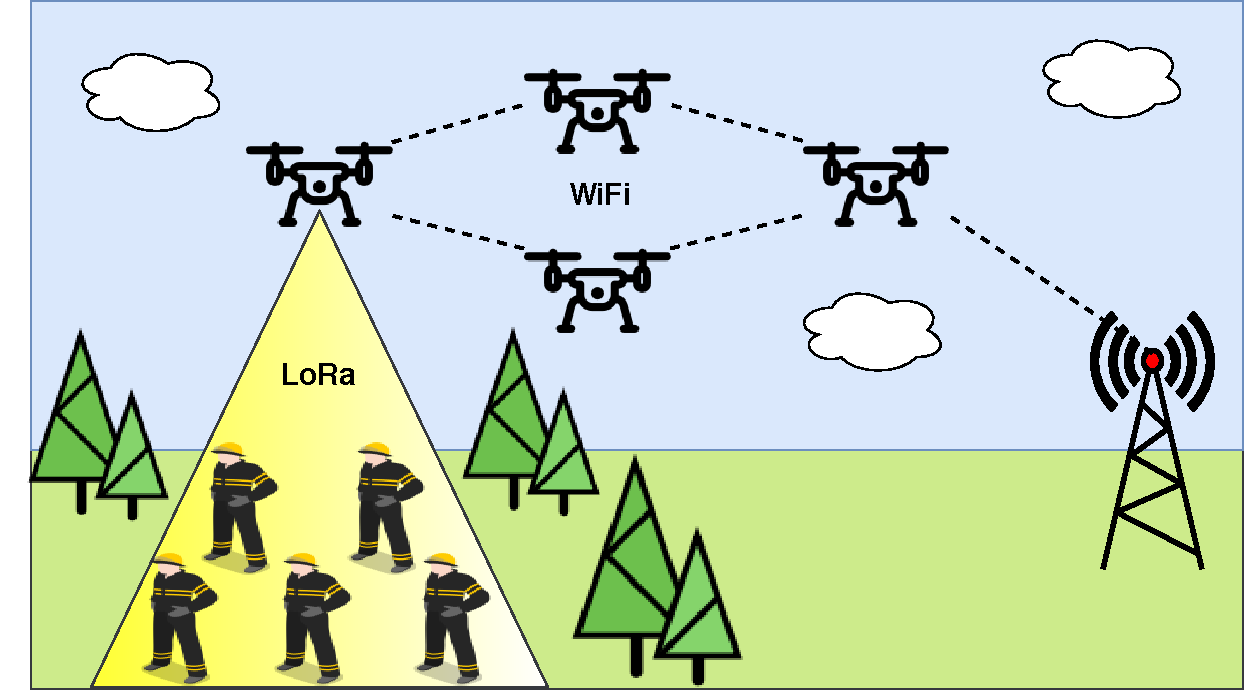
\includegraphics[width=1\textwidth]{images/system-architecture.pdf}
    \caption{Architecture of the system}
    \label{fig:system-architecture}
\end{figure}


\section{The Virtual Spring Forces Topology Algorithm}

\section{Simulation Model}

%\subsection{The ns-3 network simulator}

%\subsubsection{LoRa module}

\subsection{Propagation Models}

\subsubsection{Air-to-Ground Model}

\subsubsection{Air-to-Air Mode1l}

\subsection{Fire Fighters mobility model}

\subsection{Other parameters}